This chapter builds on the work of \cite{gettingstarted}, \cite{DoucetEstParamSSM} and \dots \todo{cite}. We will purely focus on off-line methods, that is estimating $p(x_{0:T}, \theta \vert y_{0:T})$. 

In many state-space models, both the parameters $\theta$ and the latent states $x_{1:T}$ are unknown and must be inferred simultaneously. In the previous chapter, we used the notation $p_\theta(\cdot)$ to indicate a density dependent on the parameter $\theta$. In this chapter we will use the more explicit notation $p(\cdot\vert \theta)$, as it aligns more naturally with the Bayesian framework.

In a Bayesian framework, a prior distribution $p(\theta)$ is assigned to the parameters, and inference is carried out on the joint posterior distribution given the observations $y_{1:T}$:
\begin{align}
	p(\theta,x_{1:T}\mid y_{1:T}) &= \frac{p(y_{1:T} \vert \theta, x_{1:T})\, p(\theta, x_{1:T})}{p(y_{1:T})} \nonumber \\
	&= \frac{p(y_{1:T} \vert \theta, x_{1:T})\, p(\theta)\, p(x_{1:T}\mid \theta)}{p(y_{1:T})} \nonumber \\
	&= \frac{p(y_{1:T} \vert \theta, x_{1:T})\, p(\theta)\, p(x_{1:T}\mid \theta)}{p(y_{1:T})} \nonumber \\
	&\propto p(y_{1:T} \vert \theta, x_{1:T})\, p(\theta)\, p(x_{1:T}\mid \theta),
	\label{eq:joint-posterior}
\end{align}
where 
\[
	p(y_{1:T})=\int \int p(y_{1:T}\vert \theta, x_{1:T})p(\theta)p(x_{1:T}\vert \theta)\, dx_{1:T}\, d\theta
\] 
is dropped since it is just a normalizing constant. Using the Markov structure of the \gls*{SSM} we can simplify $p(x_{1:T} \vert \theta)$ as
\[
	p(x_{1:T} \vert \theta)=p(x_1 \vert \theta)\prod_{t=2}^{T}p(x_t\vert x_{t-1}\vert \theta).
\]

When the latent states are not of primary interest, they can be integrated out to obtain the marginal posterior for the parameters:
\begin{align}
	p(\theta\mid y_{1:T}) &= \int p(\theta,x_{1:T}\mid y_{1:T})\,dx_{1:T} \nonumber \\
	&\propto p(\theta)\, p(y_{1:T} \vert \theta),
	\label{eq:marginal-posterior}
\end{align}
with the marginal likelihood defined as
\[
p(y_{1:T}\vert \theta) = \int p(x_{1:T}, y_{1:T}\vert \theta)\,dx_{1:T}.
\]

Since neither Equation (\ref{eq:joint-posterior}) or (\ref{eq:marginal-posterior}) is generally tractable, \gls*{MCMC} methods are widely used to approximate the posterior distributions. However, standard techniques such as one-variable-at-a-time Gibbs sampling tend to perform poorly for non-linear, non-Gaussian state-space models \cite{DoucetEstParamSSM}. 

\gls*{PMCMC} algorithms overcome these challenges by leveraging particle methods to construct efficient high-dimensional proposal distributions, thereby enhancing the performance of MCMC in these complex settings.

\subsection{Particle Marginal Metropolis-Hastings (PMMH)}
A \gls*{MMH} sampler would sample from the joint posterior $p(x_{1:T}, \theta \vert y_{1:T})$ by using the proposal density
\begin{equation}
	q\bigl((x_{1:T}', \theta') \vert x_{1:T}, \theta\bigr)=q(\theta'\vert \theta)p_{\theta'}(x_{1:T}' \vert y_{1:T}'),
\end{equation}
where $q(\theta' \vert \theta)$ is a proposal density to obtain a candidate parameter $\theta'$ from $\theta$, a candidate latent trajectory $x_{1:T}'$ from $x_{1:T}$, and an observation trajectory $y_{1:T}'$ from $y_{1:T}$. The acceptance probability is given by
\begin{equation}
	1 \wedge \frac{p_{\theta'}(y_{1:T})p(\theta')q(\theta \vert \theta')}{p_\theta(y_{1:T})p(\theta)q(\theta' \vert \theta)}.
\end{equation}
However, we can neither sample exactly from $p_{\theta'}(x_{1:T}' \vert y_{1:T}')$ nor compute the likelihood terms $p_{\theta'}(y_{1:T})$ and $p_{\theta}(y_{1:T})$ from the acceptance probability an implementation of \gls*{MMH} is impossible. 

A \gls*{PMMH} sampler is an approximation of the \gls*{MMH} sampler where particle methods are used to approximate these intractable terms. The pseudocode for the algorithm is given in Algorithm~\ref{algo:PMMH}. It was shown in \cite{Andrieu} that using an unbiased estimator of $\widehat{p}_\theta(y_{1:T})$ produced by the particle filter is sufficient to guarantee that the Markov chain has the correct stationary distribution for any number of particles $N$. 
% Highlight this? Very important

The proposal density $q(\theta'\vert \theta)$ is often chosen as a random walk, that is $\theta'$ 
\[q(\theta' \vert \theta) \sim N(\theta, \hat{\mathcal{P})},\]
where $\hat{\mathcal{P}}$ is the estimated posterior covariance based on a pilot run (\cite{gettingstarted}).

\begin{algorithm}[H]
	\caption{Particle Marginal Metropolis-Hastings (PMMH)}
	\label{algo:PMMH}
	\begin{algorithmic}[1]
		\State \textbf{Input:} Observation sequence \(y_{1:T}\); number of MCMC iterations \(M\); number of particles \(N\); prior density \(p(\theta)\); proposal density \(q(\theta'\mid\theta)\); and initial parameter value \(\theta^{(0)}\).
		\State \textbf{Initialization:} Set \(m \gets 0\). Run a particle filter (as explained in Chapter~\ref{chap:MCM}) with parameter \(\theta^{(0)}\) to obtain a likelihood estimate \(\widehat{p}_{\theta^{(0)}}(y_{1:T})\) and a latent state sample \(x_{1:T}^{(0)}\).
		\For{\(m=1,\dots,M\)}
		\State Propose a new parameter: \(\theta' \sim q(\theta'\mid\theta^{(m-1)})\).
		\State Run a particle filter with \(\theta'\) to obtain the likelihood estimate \(\widehat{p}_{\theta'}(y_{1:T})\) and a latent state sample \(x_{1:T}'\).
		\State Compute the acceptance probability
		\[
		\alpha = \min\Biggl\{1,\;\frac{p(\theta')\,\widehat{p}_{\theta'}(y_{1:T})\,q(\theta^{(m-1)}\mid\theta')}{p(\theta^{(m-1)})\,\widehat{p}_{\theta^{(m-1)}}(y_{1:T})\,q(\theta'\mid\theta^{(m-1)})}\Biggr\}.
		\]
		\State With probability \(\alpha\), set
		\[
		\theta^{(m)}\gets \theta',\quad x_{1:T}^{(m)}\gets x_{1:T}',\quad \widehat{p}_{\theta^{(m)}}(y_{1:T})\gets \widehat{p}_{\theta'}(y_{1:T}).
		\]
		\State Otherwise, set
		\[
		\theta^{(m)}\gets \theta^{(m-1)},\quad x_{1:T}^{(m)}\gets x_{1:T}^{(m-1)},\quad \widehat{p}_{\theta^{(m)}}(y_{1:T})\gets \widehat{p}_{\theta^{(m-1)}}(y_{1:T}).
		\]
		\EndFor	
		\State \textbf{Return:} The chain \(\{\theta^{(m)},\, x_{1:T}^{(m)}\}_{m=0}^{M}\).
	\end{algorithmic}
\end{algorithm}
Recall, that the particle filter algorithms discussed in Chapter~\ref{chap:MCM} had time complexity $O(NT)$, and thus this algorithm has time complexity $O(MNT)$. Thus, we need to decide on how to allocate computational resources for $N$ and $M$. 

The parameter \(N\) directly impacts the variance of the likelihood estimator \(\widehat{p}_\theta(y_{1:T})\). Increasing \(N\) reduces this variance, leading to a more stable acceptance probability. In practice, $N$ is typically determined via pilot runs that monitor the variance of the log-likelihood estimate, with the common guideline being to choose $N$ so that this variance is approximately around 1-1.7 when evaluated at the posterior mean of $\theta$ (\cite{Pitt} and \cite{gettingstarted}).

The number of MCMC iterations \(M\) determines the overall length of the Markov chain and hence the quality of the posterior approximation. A larger \(M\) facilitates a more thorough exploration of the posterior distribution, allowing for greater precision in the resulting parameter estimates after discarding an appropriate burn-in period. In practice, we often run several independent chains and use convergence diagnostics such as the potential scale reduction statistic, \(\hat{R}\), and the effective sample size of each parameter, see also Appendix~\ref{chp:appendixMCMC}. 


\begin{example}[SSM with unknown $\theta$]
	\label{exa:SSM_unknown_theta}
	We consider the same model from Example~\ref{exa:SSM_known_theta} and Example~\ref{exa:SSM_known_theta_cont}, that is we have $\theta=(\phi, \sigma_x, \sigma_y)$ and we have the following \gls*{SSM}
	\begin{align*}
		X_1 &\sim N(0,\, 1) \\
		X_t&=\phi X_{t-1}+\sin(X_{t-1})+\sigma_x V_t, \quad V_t \sim N(0, \, 1) \\
		Y_t&=X_t+\sigma_y W_t, \quad W_t \sim N(0, \, 1).
	\end{align*}
	We as before, set $\phi=0.7, \sigma_x=1, \sigma_y=1$, with a time horizon of $T=50$, and $N=1000$ particles. We assume $\theta$ is unknown. Thus, we need to specify priors on these three parameters. We choose the following generic weakly informative priors
	\begin{align*}
		\phi &\sim N(0,1), \\
		\sigma_x &\sim \text{half-}N(1), \\
		\sigma_y &\sim \text{half-}N(1).
	\end{align*}
	We do a prior predictive check, where we generate data from the prior and assess whether it aligns with the observed data. Data simulated from the \gls*{DGP} using the true values $\theta=(0.7, 1, 1)$ and four times from the prior is visualized in Figure~\ref{fig:Prior_predictive_check}. We see that the priors are reasonable, but note that if $\lvert \phi \rvert>1$ by the nature of the \gls*{DGP} that the observations can easily explode.  
	
	% Should I define prior predictive check and posterior predictive check?
	\begin{figure}
		\centering
		\textbf{Prior predictive check}
		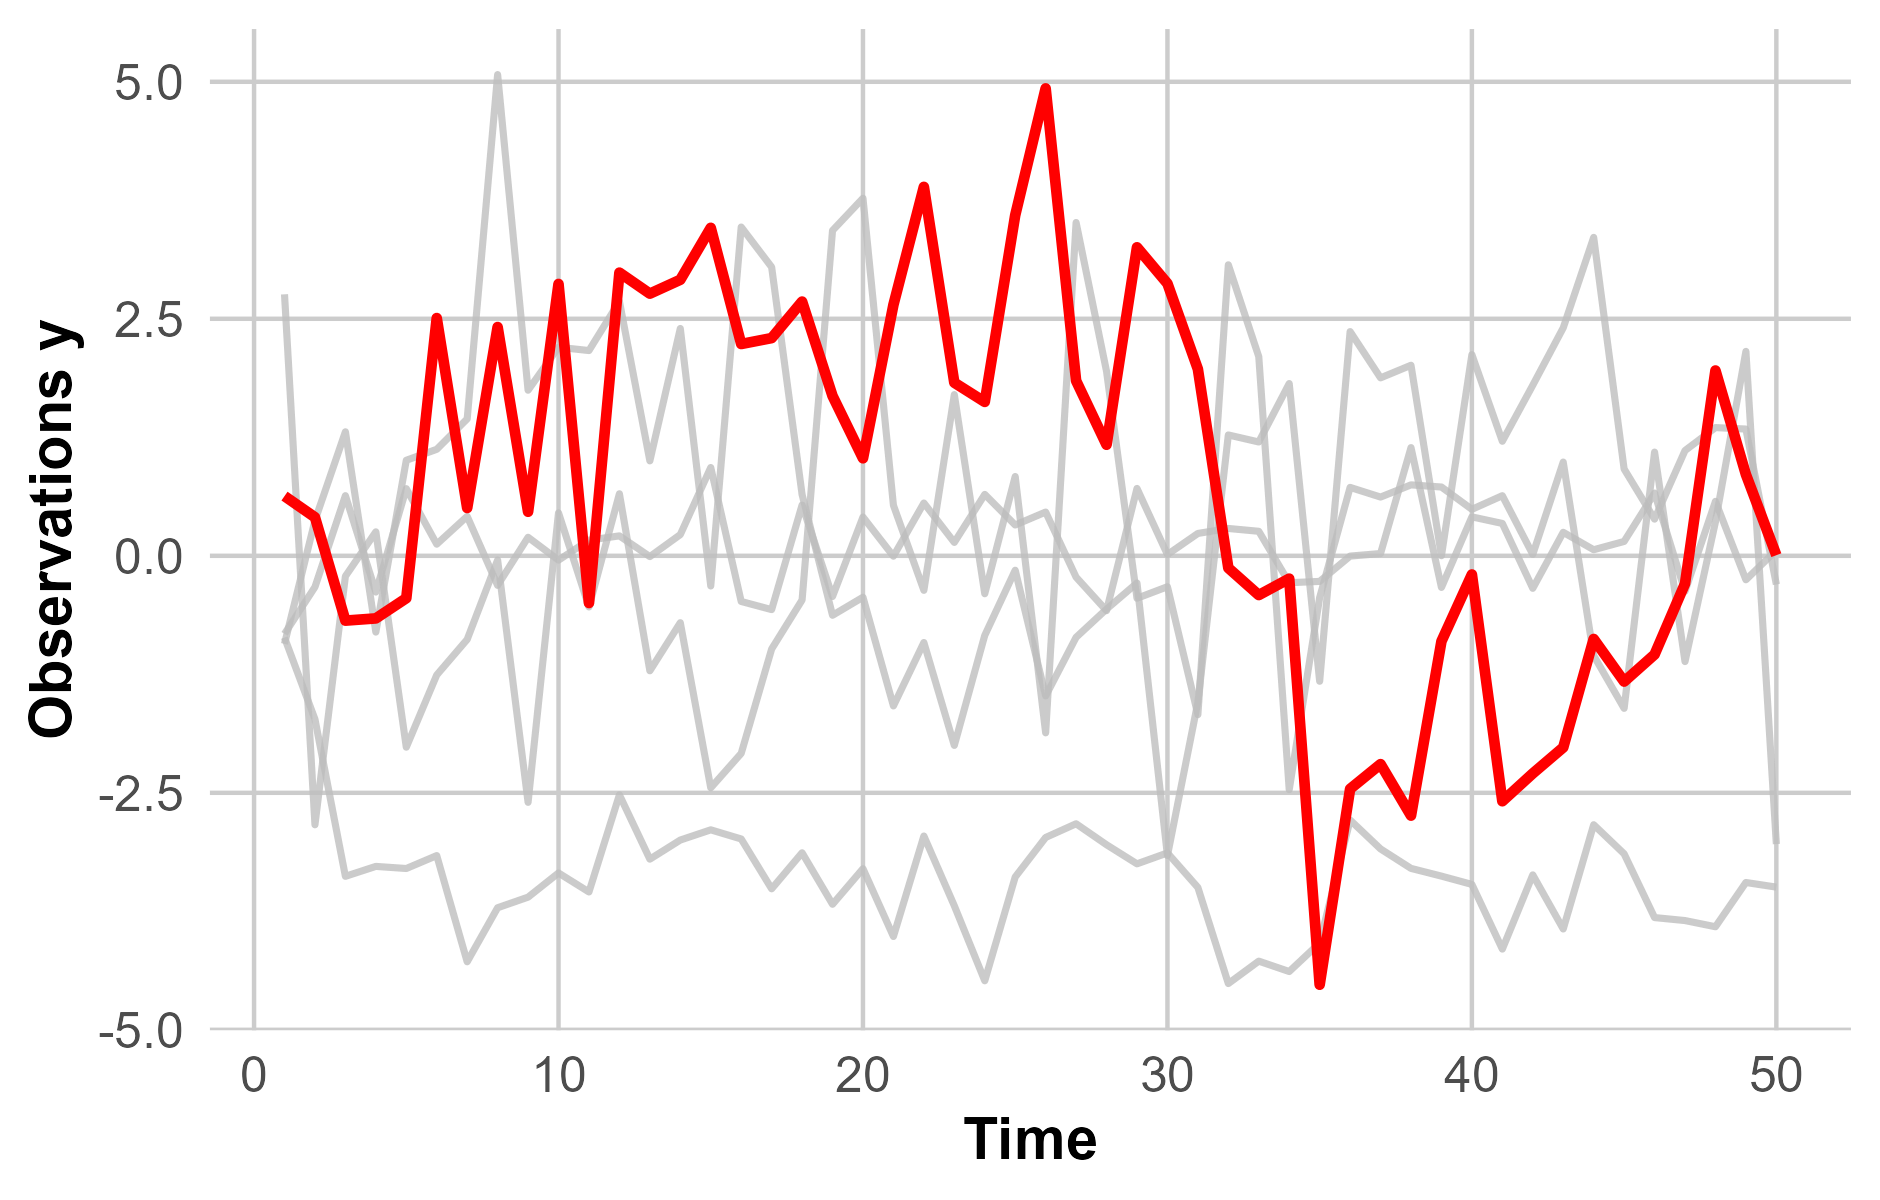
\includegraphics{prior_predictive_check.png}
		\caption{A simulated trajectory of the SSM in Example~\ref{exa:SSM_unknown_theta} alongside four simulated trajectories using the priors.}
		\label{fig:Prior_predictive_check}
		% Convert to pdf see https://www.overleaf.com/learn/latex/Inserting_Images Generating high-res and low-res images
	\end{figure}
	
	We use the proposal distribution
	\[
	q_{\text{pilot}}(\theta' \vert \theta) \sim N(\theta, 0.1 \cdot I),
	\]
	for a pilot run with $N_{\text{pilot}}=100$ particles and $M_{\text{pilot}}=2000$ \gls*{MCMC} iterations, discarding the first $1000$ samples as burn-in, and initializing $\theta$ from the priors. From this pilot run, we estimate both the posterior covariance matrix, $\hat{\mathcal{P}}$, and the posterior mean, $\hat{\theta}$. Next, using the estimated posterior mean, we calculate an estimate of the variance of the log-likelihood, denoted by $\widehat{\text{Var}}(\ell)$, by performing 10 repetitions with $N_{\text{pilot}}=100$ particles each time. Finally, we set
	\[
	N = \max\Bigl( N_{\text{pilot}} \cdot \widehat{\text{Var}}(\ell), \, 100 \Bigr),
	\]
	so that the log-likelihood has approximately unit variance at the estimated posterior while ensuring that $N$ is at least 100.
	
	We then run four independent \gls*{MCMC} chains with the proposal distribution
	\[
	q(\theta' \vert \theta) \sim N(\theta, \hat{\mathcal{P}}),
	\]
	for $M=15000$ \gls*{MCMC} iterations, discarding the first $2000$ samples as burn-in, using the value of $N$ from above and initializing $\theta$ as $\hat{\theta}$. The R code implementing this can be found at \url{https://github.com/BjarkeHautop/master-thesis/tree/main/R}; see also Appendix~\ref{chap:NumericalTricks} for further implementation details.
	
	An example chain is shown in Appendix~\ref{chap:supplementary_figures} in Figure~\ref{fig:chain}, where we see no clear signs that the chain has not converged and is not mixing well. To ensure that the posterior distribution produces data consistent with the observed data, we perform a posterior predictive check, shown in Figure~\ref{fig:Posterior_predictive_check}. The results appear reasonable, with the posterior values aligning well with the observed data.
	
	\begin{figure}
		\centering
		\textbf{Posterior predictive check}
		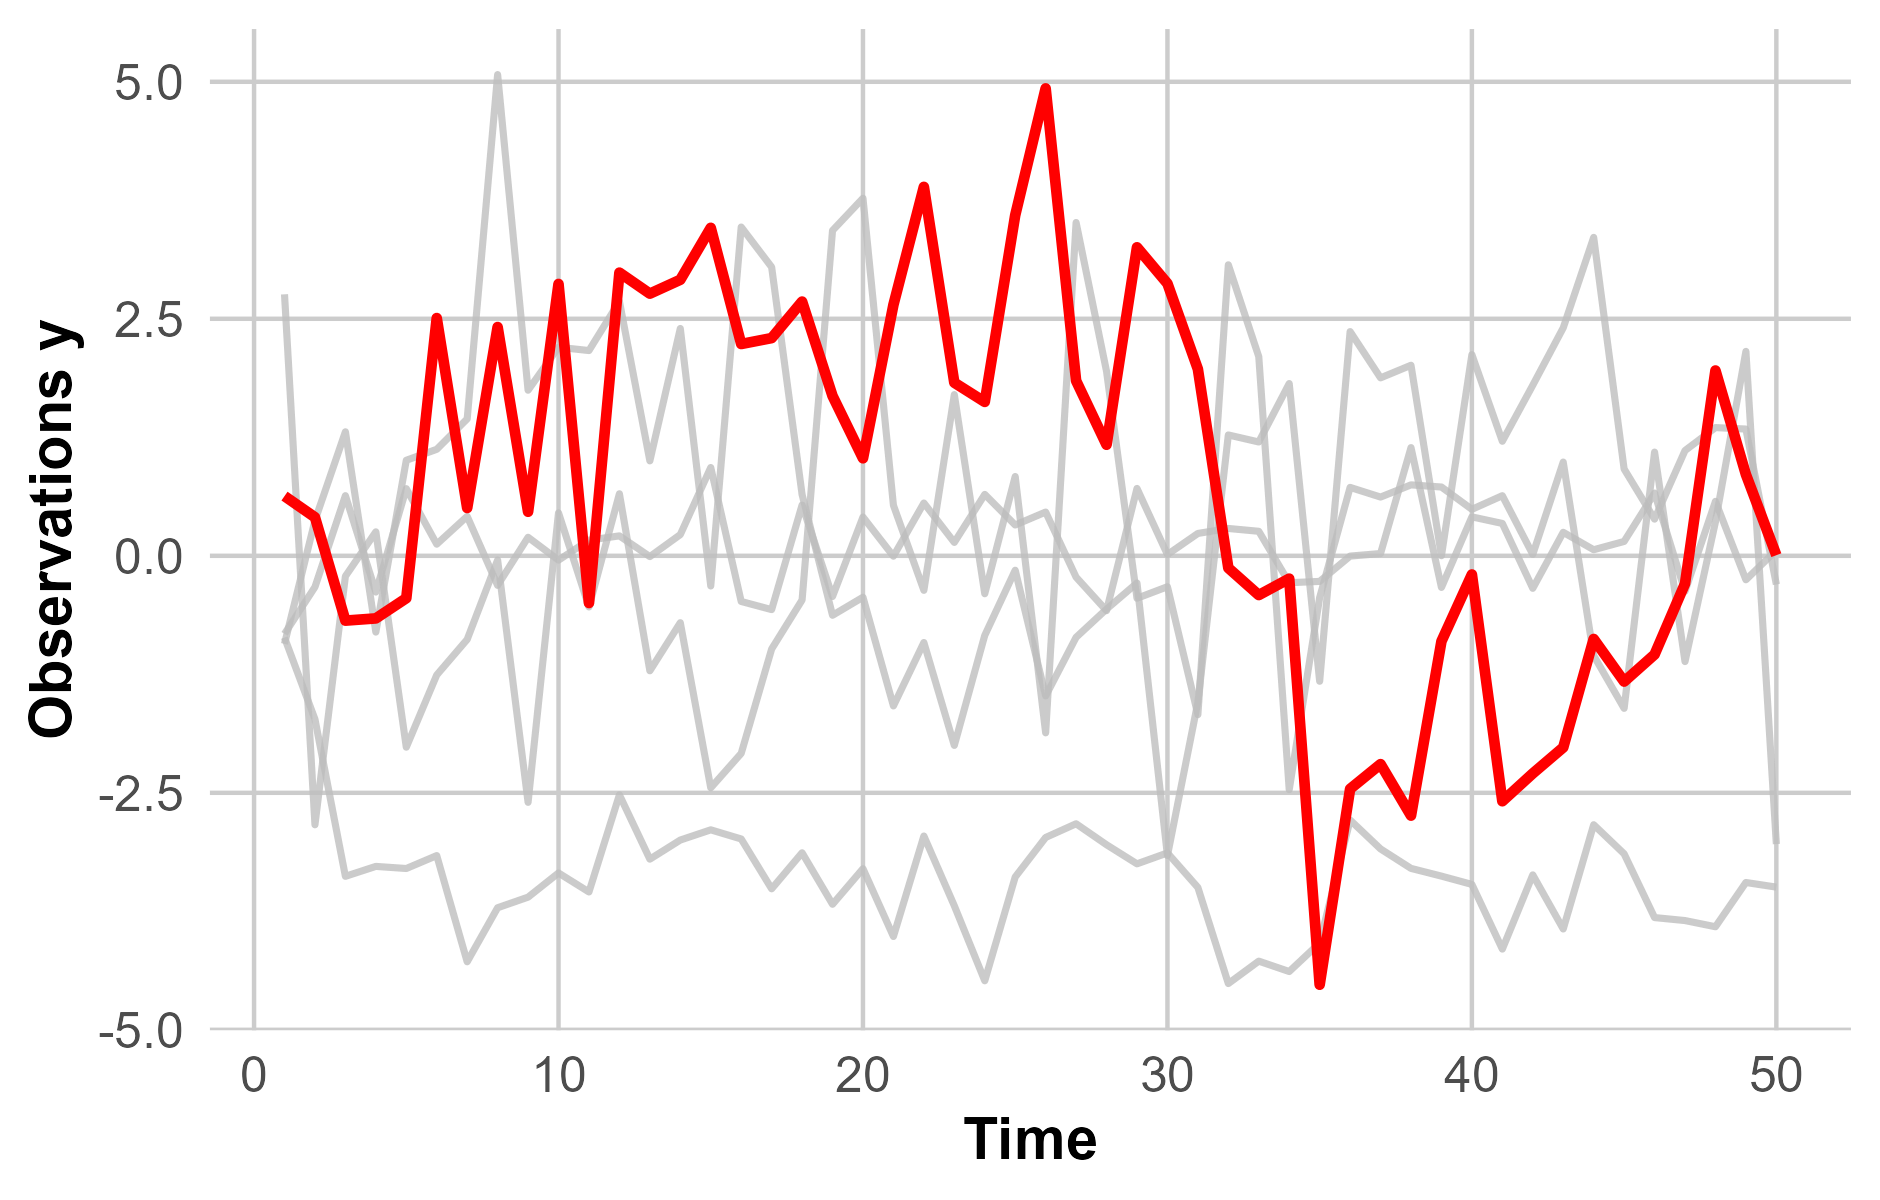
\includegraphics[width=\textwidth]{prior_predictive_check.png}
		\caption{A simulated trajectory of the SSM in Example~\ref{exa:SSM_unknown_theta} alongside four sample paths generated from the posterior predictive distribution.}
		\label{fig:Posterior_predictive_check}
		% Convert to pdf see https://www.overleaf.com/learn/latex/Inserting_Images Generating high-res and low-res images
	\end{figure} 
	
	To ensure that the chains agree and have converged to the same posterior we in Figure~\gls*{ESS} show the density plot of the four chains for $\phi$ (the figures for $\sigma_x$ and $\sigma_y$ can be found in \ref{chap:supplementary_figures}). We see that the four chains look very similar. We furthermore verify that we can trust the inference by computing the split-$\widehat{R}$ statistic and \gls*{ESS} (see Appendix~\ref{chp:appendixMCMC} for definition of these), which is summarized in Table~\ref{tab:diagnostics}. We see, that the ESS is much larger than the recommendation of at least 400 and the split-\(\widehat{R}\) are all below the recommended $1.01$. Thus, we can use the MCMC samples for reliable inference.
	
	\begin{figure}
		\centering
		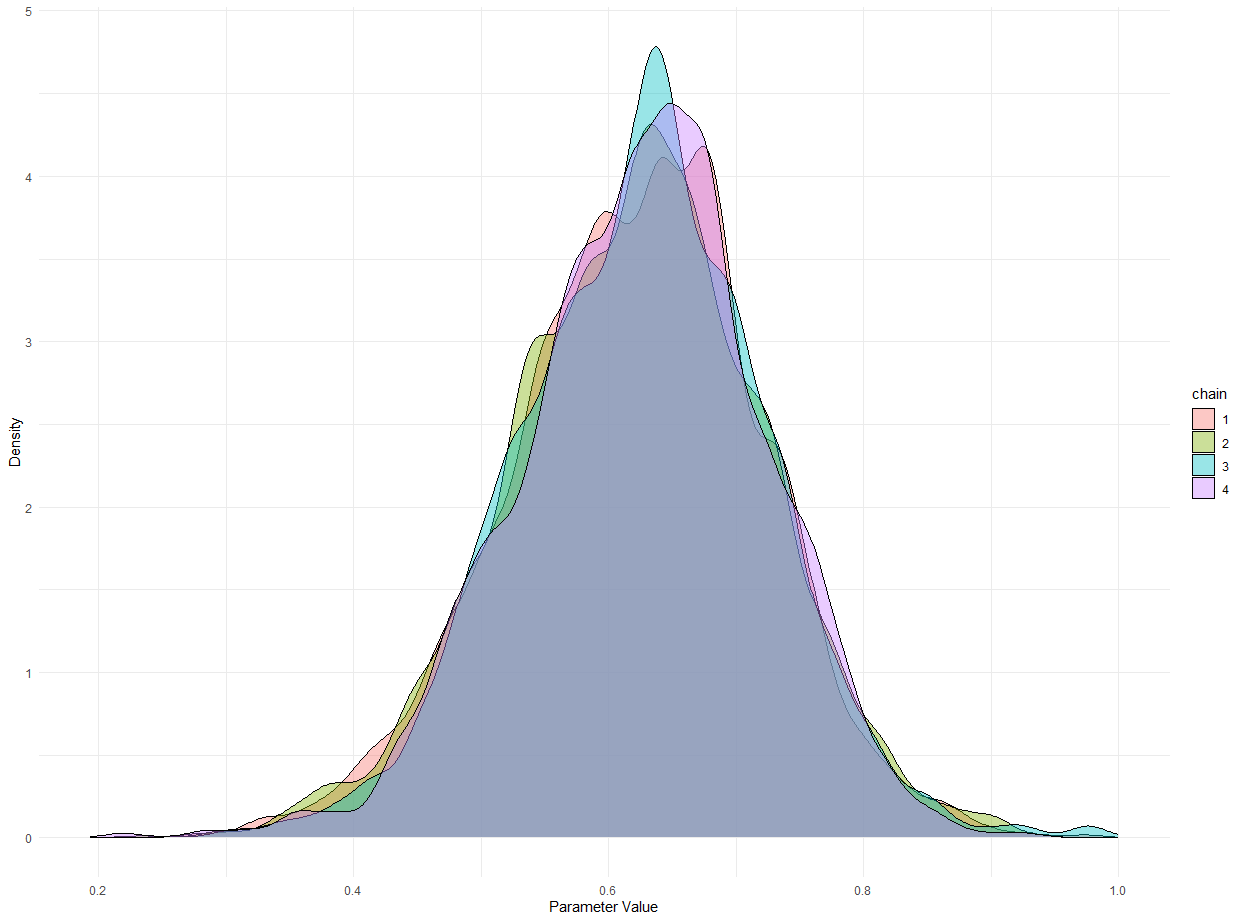
\includegraphics[width=\textwidth]{phi_density_plot.png}
		\caption{Density plot of the four chains for $\phi$ in Example~\ref{exa:SSM_unknown_theta}.
		\textbf{UPDATE FIGURE TO HIGH QUALITY}}
		\label{fig:phi_dens}
	\end{figure}
	
	\begin{table}
		\centering
		\caption{ESS and split-\(\widehat{R}\) for \(\phi\), \(\sigma_x\), and \(\sigma_y\)}
		\label{tab:diagnostics}
		\begin{tabular}{lcc}
			\toprule
			Parameter & ESS & split-\(\widehat{R}\) \\
			\midrule
			\(\phi\)       & 2609  & 1.002 \\
			\(\sigma_x\)   & 1806  & 1.002 \\
			\(\sigma_y\)   & 1304  & 1.003 \\
			\bottomrule
		\end{tabular}
	\end{table}
	
	The posterior mean and $95\%$ credible intervals are given in Table~\ref{tab:mean_credible_interval}. The RMSE of the latent state was $0.79$, only slightly worse than the result of the filtering and smoothing algorithms from Table~\ref{tab:performance_ext}, where the parameters were known. \textbf{ONLY BASED ON 1 SAMPLE}
	\begin{table}
		\centering
		\caption{Mean and Credible Interval for Parameters}
		\label{tab:mean_credible_interval}
		\begin{tabular}{lcc}
			\toprule
			Parameter & Mean & 95\% Credible Interval \\
			\midrule
			\(\phi\)       & 0.62  & [0.42, 0.81] \\
			\(\sigma_x\)   & 1.01  & [0.64, 1.49] \\
			\(\sigma_y\)   & 0.89  & [0.45, 1.29] \\
			\bottomrule
		\end{tabular}
	\end{table}
\end{example}


